\section{Experiments}
\label{sec:experiments}

\cref{sec:experiments-benchmark} benchmarks \methodabbrv{} against the LSSL and efficient Transformer models.
\cref{sec:experiments-lrd} validates \methodabbrv{} on LRDs: the LRA benchmark and raw speech classification.
\cref{sec:experiments-general} investigates whether \methodabbrv{} can be used as a general sequence model to perform effectively and efficiently in a wide variety of settings including image classification, image and text generation, and time series forecasting.

\subsection{\methodabbrv{} Efficiency Benchmarks}
\label{sec:experiments-benchmark}
We benchmark that \methodabbrv{} can be trained quickly and efficiently, both compared to the LSSL, as well as efficient Transformer variants designed for long-range sequence modeling.
As outlined in \cref{sec:s4}, \methodabbrv{} is theoretically much more efficient than the LSSL, and \cref{tab:ssm-benchmark} confirms that the \methodabbrv{} is orders of magnitude more speed- and memory-efficient for practical layer sizes.
In fact, \methodabbrv's speed and memory use is competitive with the most efficient Transformer variants benchmarked by \citet{tay2021long}---Linear Transformer~\citep{katharopoulos2020transformers} and Performer~\citep{choromanski2020rethinking}---in a parameter-matched setting (\cref{tab:lra-benchmark}, following the protocol of \citet{tay2021long}).


\begin{figure}[t!]
  \begin{minipage}[t]{0.54\linewidth}
    \small
    \centering
    \captionsetup{type=table}
    \caption{Deep SSMs: The \methodabbrv{} parameterization with \cref{alg:s4-convolution} is asymptotically more efficient than the LSSL.}
    \resizebox{\linewidth}{!}{
      \begin{tabular}{@{}llllllllll@{}}
        \toprule
        & \multicolumn{3}{c}{\textsc{Training Step (ms)}} & \multicolumn{3}{c}{\textsc{Memory Alloc. (MB)}} \\
        \cmidrule{2-4} \cmidrule{5-7}
        Dim.        & 128                                         & 256                                        & 512                                        & 128   & 256  & 512    \\
        \midrule
        LSSL        & 9.32                                        & 20.6                                       & 140.7                                      & 222.1 & 1685 & 13140  \\
        \textbf{\methodabbrv} & 4.77                                        & 3.07                                       & 4.75                                       & 5.3   & 12.6 & 33.5   \\
        \midrule
        Ratio & \( 1.9\times \) & \( 6.7\times \) & \( \bm{29.6}\times \) & \( 42.0\times \) & \( 133\times \) & \( \bm{392\times} \) \\
        \bottomrule
      \end{tabular}%
    }
    \label{tab:ssm-benchmark}
  \end{minipage}
  \hfill
  \begin{minipage}[t]{0.45\linewidth}
    \small
    \captionsetup{type=table}
    \centering
    \caption{Benchmarks vs. efficient Transformers}
    \resizebox{\linewidth}{!}{
      \begin{tabular}{@{}lllll@{}}
        \toprule
                              & \multicolumn{2}{c}{\textsc{Length 1024}} & \multicolumn{2}{c}{\textsc{Length 4096}} \\
        \cmidrule{2-3} \cmidrule{4-5}
                              & Speed                                    & Mem.                                      & Speed                        & Mem.                          \\
        \midrule
        Transformer           & 1\( \times \)                            & 1\( \times \)                             & 1\( \times \)                & 1\( \times \)                 \\
        \midrule
        Performer             & 1.23\( \times \)                         & \underline{0.43}\( \times \)              & 3.79\( \times \)             & \underline{0.086}\( \times \) \\
        Linear Trans.         & \textbf{1.58}\( \times \)                & \textbf{0.37}\( \times \)                 & \textbf{5.35}\( \times \)    & \textbf{0.067}\( \times \)    \\
        \midrule
        \textbf{\methodabbrv} & \textbf{1.58}\( \times \)                & \underline{0.43}\( \times \)              & \underline{5.19}\( \times \) & 0.091\( \times \)             \\
        \bottomrule
      \end{tabular}%
    }
    \label{tab:lra-benchmark}
  \end{minipage}
\end{figure}

\subsection{Learning Long Range Dependencies}
\label{sec:experiments-lrd}
As described in \cref{sec:ss-memory,sec:s4-motivation}, \methodabbrv{} uses a principled approach to address LRDs based on the HiPPO theory of continuous-time memorization.
Our goal in this section is to validate that \methodabbrv{} achieves high performance on difficult tasks that require long-range reasoning.
We focus here on two problems:
(i) the Long-Range Arena, a well-known benchmark designed to test efficient sequence models on LRDs, and
(ii) a speech classification problem as a real-world test of LRDs.


\begin{figure}[t!]
  \centering
    \begin{subfigure}{0.3\linewidth}
        \centering
        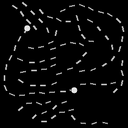
\includegraphics[width=\linewidth]{figs/pathx_positive.png}
    \end{subfigure}%
    \quad
    \begin{subfigure}{0.58\linewidth}
        \centering
        \lineskip=0pt
        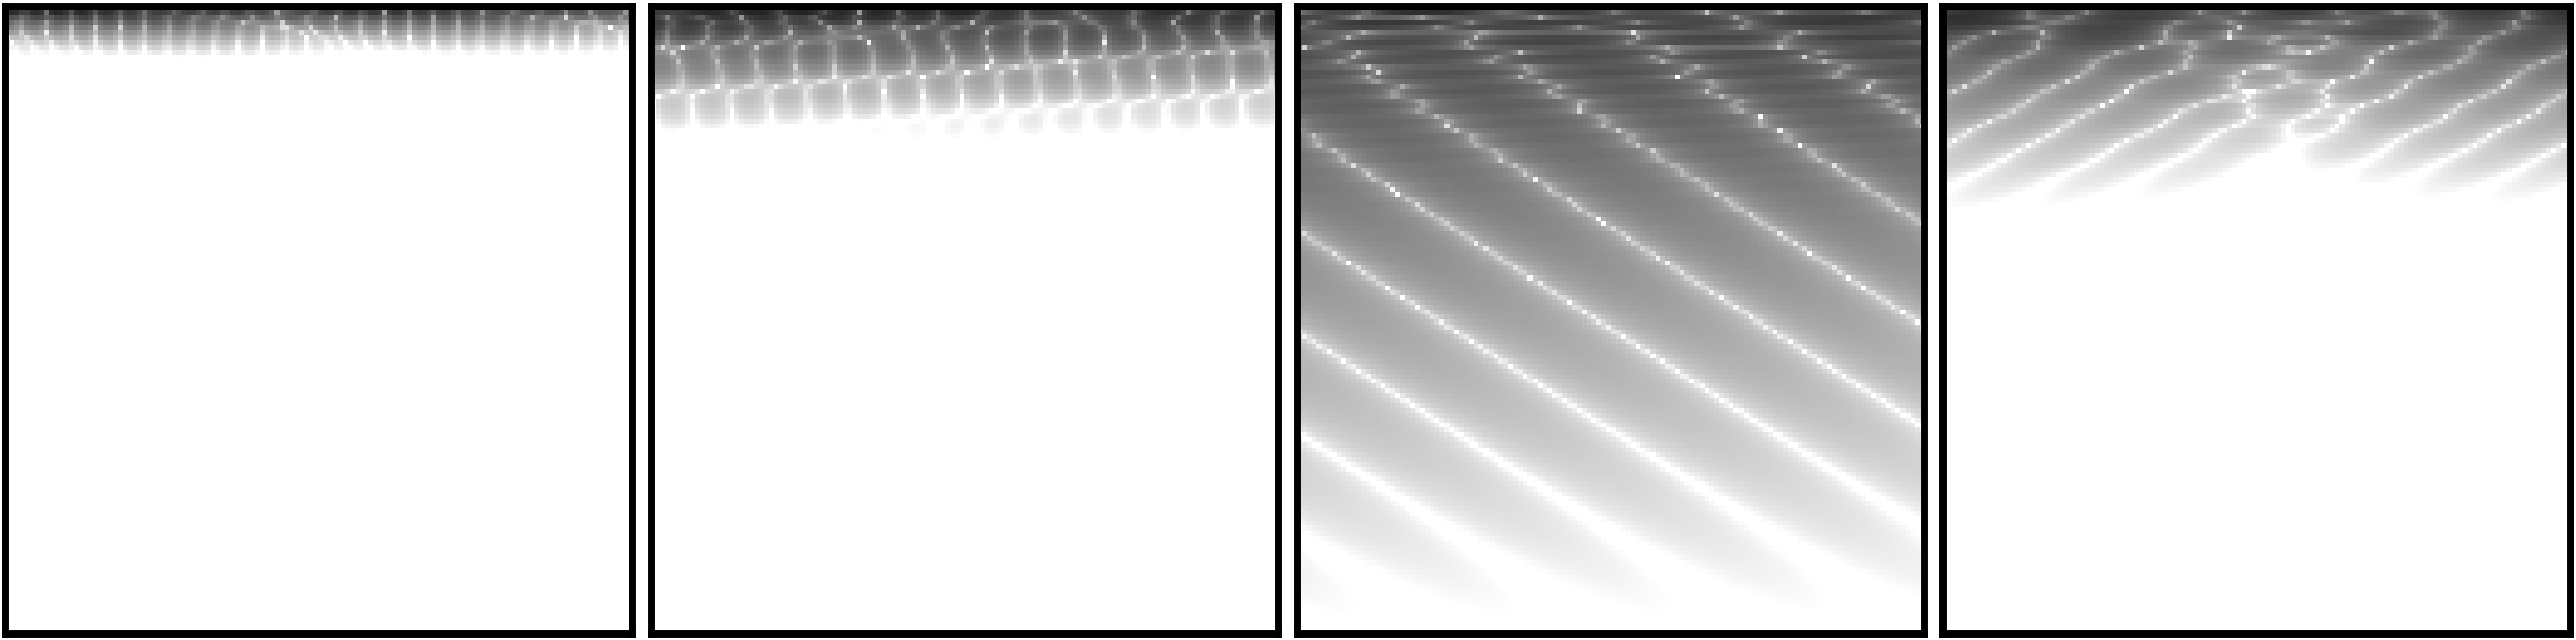
\includegraphics[width=\linewidth]{figs/pathfinder_4_filters_layer_0.png}\\
        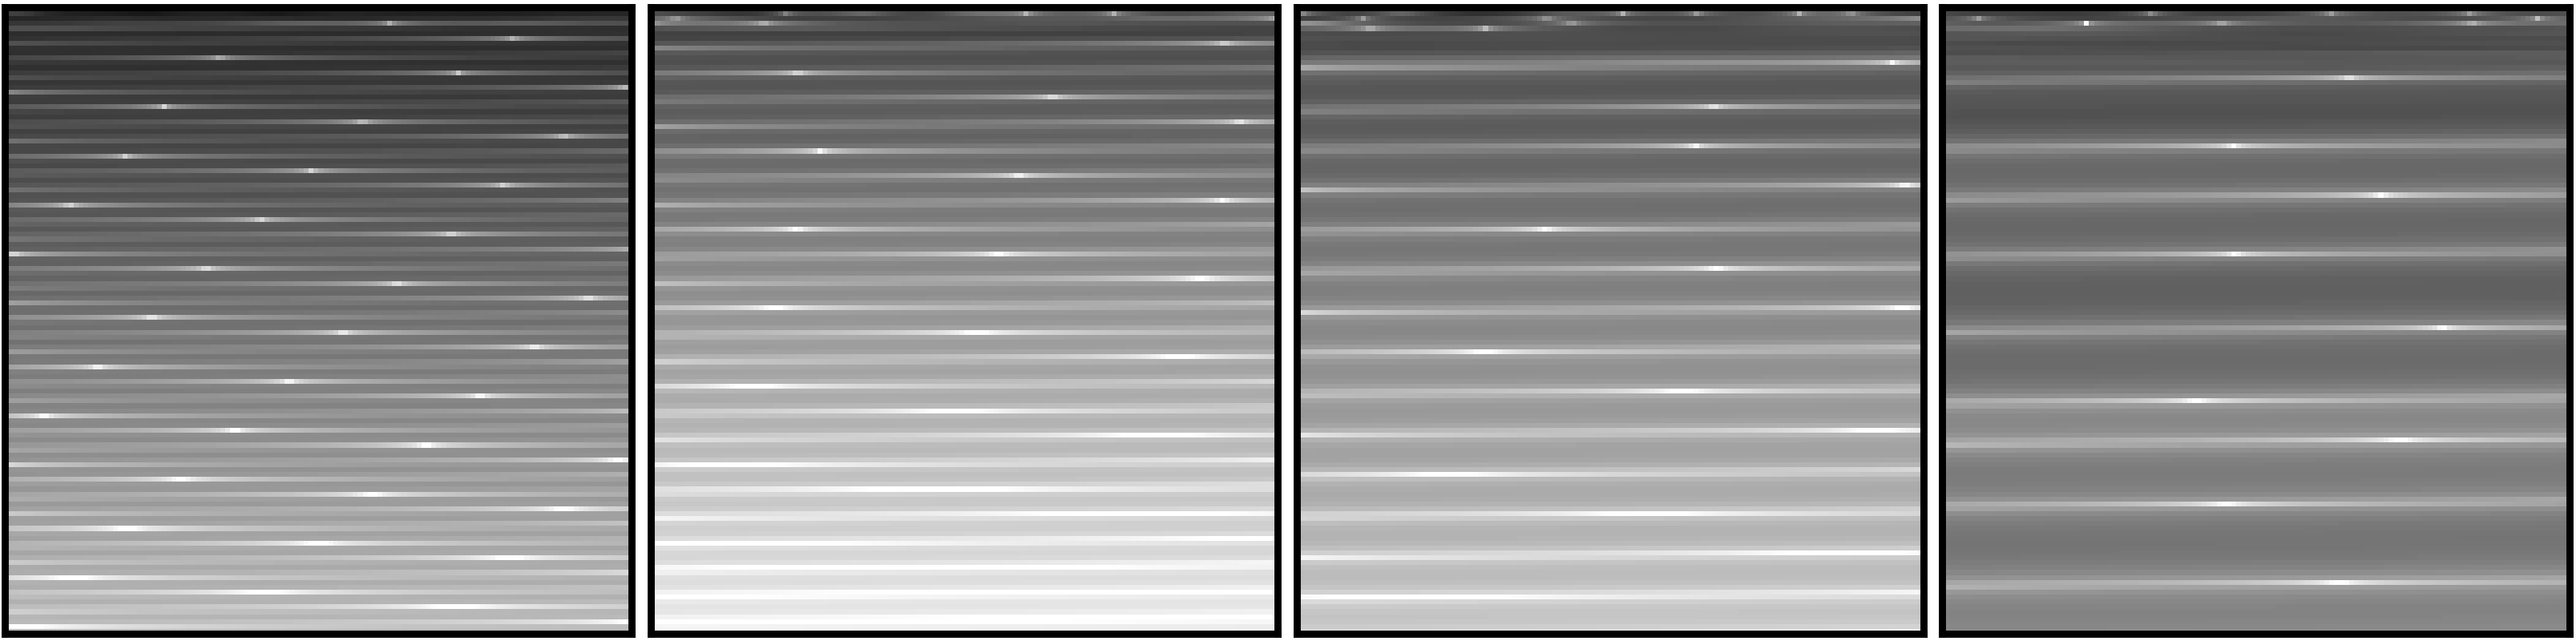
\includegraphics[width=\linewidth]{figs/pathfinder_4_filters_layer_5.png}
    \end{subfigure}
      \caption{
        Visualizations of a trained \methodabbrv{} model on LRA Path-X. SSM convolution kernels \( \bm{\overline{K}} \in \mathbbm{R}^{16384} \) are reshaped into a \( 128 \times 128 \)  image. (\textit{Left}) Example from the Path-X task, which involves deducing if the markers are connected by a path (\textit{Top}) Filters from the first layer (\textit{Bottom}) Filters from the last layer.
    }
  \label{fig:pathx-filters}
\end{figure}


\begin{table}[t!]
  \small
  \caption{
    (\textbf{Long Range Arena})
    (\textit{Top}) Original Transformer variants in LRA. Full results in \cref{sec:experiment-details-lrd}.
    (\textit{Bottom}) Other models reported in the literature.
    \emph{Please read \cref{sec:reproduction} before citing this table.}
  }
    \centering
    \begin{tabular}{@{}llllllll@{}}
        \toprule
        \textsc{Model}        & \textsc{ListOps}  & \textsc{Text}     & \textsc{Retrieval} & \textsc{Image}    & \textsc{Pathfinder} & \textsc{Path-X} & \textsc{Avg}      \\
        \midrule
        Transformer           & 36.37             & 64.27             & 57.46              & 42.44             & 71.40               & \xmark          & 53.66             \\
        Reformer              & \underline{37.27} & 56.10             & 53.40              & 38.07             & 68.50               & \xmark          & 50.56             \\
        BigBird               & 36.05             & 64.02             & 59.29              & 40.83             & 74.87               & \xmark          & 54.17             \\
        Linear Trans.         & 16.13             & \underline{65.90} & 53.09              & 42.34             & 75.30               & \xmark          & 50.46             \\
        Performer             & 18.01             & 65.40             & 53.82              & 42.77             & 77.05               & \xmark          & 51.18             \\
        \midrule
        FNet                  & 35.33             & 65.11             & 59.61              & 38.67             & \underline{77.80}   & \xmark          & 54.42             \\
        Nystr{\"o}mformer     & 37.15             & 65.52             & \underline{79.56}  & 41.58             & 70.94               & \xmark          & 57.46             \\
        Luna-256              & 37.25             & 64.57             & 79.29              & \underline{47.38} & 77.72               & \xmark          & \underline{59.37} \\
        \textbf{\methodabbrv} & \textbf{59.60}    & \textbf{86.82}    & \textbf{90.90}     & \textbf{88.65}    & \textbf{94.20}      & \textbf{96.35}  & \textbf{86.09}    \\
        \bottomrule
    \end{tabular}
    \label{tab:lra}
\end{table}


\textbf{Long Range Arena (LRA).}
LRA~\citep{tay2021long} contains $6$ tasks with lengths 1K-16K steps, encompassing modalities and objectives that require similarity, structural, and visuospatial reasoning.
\cref{tab:lra} compares \methodabbrv{} against the 11 Transformer variants from \citet{tay2021long} as well as follow-up work.
%
\methodabbrv{} substantially advances the SoTA, outperforming all baselines on all tasks and averaging $80.48\%$ compared to less than \( 60\% \) for every baseline.
Notably, \methodabbrv{} solves the Path-X task, an extremely challenging task
that involves reasoning about LRDs over sequences of length \( 128\times 128 = 16384 \).
All previous models have failed (i.e.\ random guessing) due to memory or computation bottlenecks, or simply being unable to learn such long dependencies.

We analyze \methodabbrv's performance on Path-X by visualizing its learned representations,
in particular 1-D convolution kernels \( \bm{\overline{K}} \)
which are the focus of our technical results in \cref{sec:s4}.
\cref{fig:pathx-filters} shows that \methodabbrv{} learns a variety of filters that display spatially consistent structure
and demonstrate awareness of the 2-D nature of the data.
In particular, the lower layers learn simple kernels that extract features from just a few rows of local context while ignoring the rest of the image.
On the other hand, higher layers aggregate information globally across full columns of the image at varying spatial frequencies.
Filters in these higher layers span the entire context ($16384$ pixels), confirming \methodabbrv's ability to learn LRDs.



\begin{figure}[b!]
\begin{minipage}[t]{0.47\linewidth}
  \small
  \centering
  \captionsetup{type=table}
  \caption{
    (\textbf{SC10 classification})
    Transformer, CTM, RNN, CNN, and SSM models.
    (\textit{MFCC}) Standard pre-processed MFCC features (length 161).
    (\textit{Raw}) Unprocessed signals (length 16000).
    (\( \mathit{0.5\times} \)) Frequency change at test time.
    \xmark{} denotes not applicable or computationally infeasible on single GPU.
    \emph{Please read \cref{sec:reproduction} before citing this table.}
  }
  \vspace*{-5pt}
  \begin{tabular}{@{}llllllllll@{}}
    \toprule
                 & \textsc{MFCC}     & \textsc{Raw}      & \( 0.5\times \)   \\
    \midrule
    Transformer  & 90.75             & \xmark            & \xmark            \\
    Performer    & 80.85             & 30.77             & 30.68             \\
    \midrule
    ODE-RNN      & 65.9              & \xmark            & \xmark            \\
    NRDE         & 89.8              & 16.49             & 15.12             \\
    \midrule
    ExpRNN       & 82.13             & 11.6              & 10.8              \\
    LipschitzRNN & 88.38             & \xmark            & \xmark            \\
    \midrule
    CKConv       & \textbf{95.3}     & 71.66             & \underline{65.96} \\
    WaveGAN-D    & \xmark            & \underline{96.25} & \xmark            \\
    \midrule
    LSSL         & 93.58             & \xmark            & \xmark            \\
    \textbf{\methodabbrv}  & \underline{93.96} & \textbf{98.32}    & \textbf{96.30}    \\
    \bottomrule
  \end{tabular}
  \label{tab:sc}
\end{minipage}
\hfill
\begin{minipage}[t]{0.47\linewidth}
  \small
  \centering
  \captionsetup{type=table}
  \caption{
    (\textbf{Pixel-level 1-D image classification})
    Comparison against reported test accuracies from prior works (Transformer, RNN, CNN, and SSM models).
    Extended results and citations in \cref{sec:experiment-details}.
  }
  \begin{tabular}{@{}llll@{}}
    \toprule
                     & \textsc{sMNIST} & \textsc{pMNIST}   & \textsc{sCIFAR}   \\
    \midrule
    Transformer      & 98.9            & 97.9              & 62.2              \\
    \midrule
    LSTM             & 98.9            & 95.11             & 63.01             \\
    r-LSTM           & 98.4            & 95.2              & 72.2              \\
    UR-LSTM          & 99.28           & 96.96             & 71.00             \\
    UR-GRU           & 99.27           & 96.51             & 74.4              \\
    HiPPO-RNN        & 98.9            & 98.3              & 61.1              \\
    LMU-FFT          & -               & 98.49             & -                 \\
    LipschitzRNN     & 99.4            & 96.3              & 64.2              \\
    \midrule
    TCN              & 99.0            & 97.2              & -                 \\
    TrellisNet       & 99.20           & 98.13             & 73.42             \\
    CKConv           & 99.32           & 98.54             & 63.74             \\
    \midrule
    LSSL & \underline{99.53}           & \textbf{98.76}    & \underline{84.65} \\
    \textbf{\methodabbrv}      & \textbf{99.63}  & \underline{98.70} & \textbf{91.13}    \\
    \bottomrule
  \end{tabular}
  \label{tab:image}
\end{minipage}
\end{figure}

\textbf{Raw Speech Classification.}
Speech is a typical real-world time series domain, involving signals sampled from an underlying physical process at high frequency.
%
We perform speech classification using the SC10 subset of the \emph{Speech Commands} dataset~\citep{Warden2018SpeechCA} (see \cref{sec:reproduction}).
While most sequence models for speech rely on extensive preprocessing (e.g. to MFCC features), we classify raw speech (length-$16000$) following~\citet{romero2021ckconv}.
%
\methodabbrv{} achieves $98.3\%$ accuracy, higher than all baselines that use the $100\times$ shorter MFCC features, and validates that a powerful LRD model is able to extract more information from the raw data and outperform hand-crafted pre-processing.
Additionally, we include a baseline CNN specifically designed for raw speech, the discriminator from the WaveGAN model~\citep{Donahue2019AdversarialAS},
which performs worse than \methodabbrv{} while having $90\times$ more parameters and incorporating many more
architectural heuristics (\cref{sec:experiment-details-lrd}).

\subsection{\methodabbrv{} as a General Sequence Model}
\label{sec:experiments-general}

A key goal of sequence modeling research is to develop a single model that can be applied in many domains (e.g. images, audio, text, time-series) with a broad range of capabilities (e.g. efficient training, fast generation, handling irregularly sampled data).
As a fundamental scientific model, SSMs are a promising candidate that come with a range of capabilities, and \methodabbrv's strong results on LRD benchmarks spanning images, text, and speech are evidence of \methodabbrv's potential as a general sequence model.
In this section, we focus on understanding this question in more depth by highlighting key strengths of \methodabbrv{} in settings that usually require specialized models.
The tasks we focus on (generative modeling, image classification, time-series forecasting)
are considered as LRD tasks in the literature,
and serve as additional validation that \methodabbrv{} handles LRDs efficiently.


\textbf{Large-scale generative modeling.}
We investigate two well-studied image and text benchmarks to validate the scalability, flexibility, and efficiency of \methodabbrv.
These tasks require much larger models than our previous tasks -- up to $250$M parameters.

First, CIFAR density estimation is a popular benchmark for autoregressive models, where images are flattened into a sequence of $3072$ RGB subpixels that are predicted one by one.
\cref{tab:cifar-generation} shows that \emph{with no 2D inductive bias}, \methodabbrv{} is competitive with the best models designed for this task.

Second, WikiText-103 is an established benchmark for language modeling, an important task for large-scale sequence models where tokens are predicted sequentially based on past context.
Although RNNs were the model of choice for many years, Transformers are now the dominant model in such applications that contain data that is inherently discrete.
We show that alternative models to Transformers can still be competitive in these settings.
By simply taking a strong Transformer baseline \citep{baevski2018adaptive} and replacing the self-attention layers,
\methodabbrv{} substantially closes the gap to Transformers (within $0.8$ ppl), setting SoTA for attention-free models by over $2$ ppl.

\textbf{Fast autoregressive inference.}
A prominent limitation of autoregressive models is inference speed (e.g. generation),
since they require a pass over the full context for every new sample.
Several methods have been specifically crafted to overcome this limitation such as the Linear Transformer, a hybrid Transformer/RNN that switches to a stateful, recurrent view at inference time for speed.

As a stateful model, SSMs automatically have this ability (\cref{fig:properties}).
By switching to its recurrent representation (\cref{sec:ss-recurrent}),
\methodabbrv{} requires \emph{constant memory and computation} per time step -- in contrast to standard autoregressive models which scale in the context length.
On both CIFAR-10 and WikiText-103,
we report the throughput of various models at generation time, with \methodabbrv{} around $60\times$ faster than a vanilla Transformer on both tasks (details in \cref{sec:experiment-details-general-speed}).


\textbf{Sampling resolution change.}
As a continuous-time model, \methodabbrv{} automatically adapts to data sampled at different rates,
a challenging setting for time series with a dedicated line of work \citep{rubanova2019latent,de2019gru,romero2021ckconv}.
Without re-training, \methodabbrv{} achieves $96.3\%$ accuracy at $0.5\times$ the frequency on Speech Commands 10 (\cref{tab:sc}), simply by changing its internal step size \( \dt \) (\cref{sec:ss-recurrent}).


\begin{figure}
\begin{minipage}[t]{0.525\linewidth}
  \small
  \centering
  \captionsetup{type=table}
  \caption{
    (\textbf{CIFAR-10 density estimation})
    As a generic \mbox{sequence} model, \methodabbrv{} is competitive with previous autoregressive models (in bits per dim.) while incorporating no 2D inductive bias,
    and has fast generation through its recurrence mode.
  }
  \vspace*{-4pt}
  \resizebox{\linewidth}{!}{
    \begin{tabular}{@{}lllll@{}}
      \toprule
      Model               & bpd              & 2D bias          & Images / sec                           \\
      \midrule
      Transformer         & 3.47             & \textbf{None}    & 0.32 (\( 1\times \))                   \\
      Linear Transf.       & 3.40             & \textbf{None}    & 17.85 (\( 56\times \))     \\
      PixelCNN           & 3.14             & 2D conv.         & -                                      \\
      Row PixelRNN        & 3.00             & 2D BiLSTM        & -                                      \\
      PixelCNN++          & 2.92             & 2D conv.         & \underline{19.19} (\( 59.97\times \))              \\
      Image Transf.       & 2.90             & 2D local attn.   & 0.54 (1.7$\times$)                     \\
      PixelSNAIL          & \underline{2.85} & 2D conv. + attn. & 0.13 (0.4$\times$)                     \\
      Sparse Transf.      & \textbf{2.80}    & 2D sparse attn.  & -                                      \\
      \midrule
      \textbf{\methodabbrv} (base)  & 2.92             & \textbf{None}    & \textbf{20.84} (\( \bm{65.1\times} \)) \\
      \textbf{\methodabbrv} (large) & \underline{2.85} & \textbf{None}    & 3.36 (\( 10.5\times \))                \\
      \bottomrule
    \end{tabular}
  }
  \label{tab:cifar-generation}
\end{minipage}
\hfill
\begin{minipage}[t]{0.47\linewidth}
  \small
  \centering
  \captionsetup{type=table}
  \caption{
    (\textbf{WikiText-103 language modeling})
    \methodabbrv{} approaches the performance of Transformers with much faster generation.
    (\textit{Top}) Transformer baseline which our implementation is based on, with attention replaced by \methodabbrv.
    (\textit{Bottom}) Attention-free models (RNNs and CNNs).
  }
  \resizebox{\linewidth}{!}{
    \begin{tabular}{@{}llll@{}}
      \toprule
      Model         & Params & Test ppl.      & Tokens / sec                       \\
      \midrule
      Transformer   & 247M   & \textbf{20.51} & 0.8K (\( 1\times \))               \\
      \midrule
      GLU CNN       & 229M   & 37.2           & -                                  \\
      AWD-QRNN      & 151M   & 33.0           & -                                  \\
      LSTM + Hebb.  & -      & 29.2           & -                                  \\
      TrellisNet    & 180M   & 29.19          & -                                  \\
      Dynamic Conv. & 255M   & 25.0           & -                                  \\
      TaLK Conv.    & 240M   & 23.3           & -                                  \\
      \textbf{\methodabbrv}   & 249M   & \textbf{20.95} & \textbf{48K} (\( \bm{60\times} \)) \\
      \bottomrule
    \end{tabular}
  }
  \label{tab:wt103}
\end{minipage}
\end{figure}


\begin{table*}[!b]
\caption{Univariate long sequence time-series forecasting results. Full results in \cref{sec:experiment-details-general-informer}.}
\centering
\resizebox{\linewidth}{!}{
  \begin{tabular}{@{}llllllllllll@{}}
    \toprule
                 & \textbf{\methodabbrv}          & {Informer}        & {LogTrans}   & {Reformer}   & {LSTMa}      & {DeepAR}     & {ARIMA}      & {Prophet}    \\
    \midrule
                 & MSE~~MAE                       & MSE~~MAE          & MSE~~MAE     & MSE~~MAE     & MSE~~MAE     & MSE~~MAE     & MSE~~MAE     & MSE~~MAE     \\
    \midrule
    {{ETTh$_1$}} & \textbf{0.116}~~\textbf{0.271} & 0.269~~0.435      & 0.273~~0.463 & 2.112~~1.436 & 0.683~~0.768 & 0.658~~0.707 & 0.659~~0.766 & 2.735~~3.253 \\
    {{ETTh$_2$}} & \textbf{0.187}~~\textbf{0.358} & {0.277}~~{0.431} & 0.303~~0.493 & 2.030~~1.721 & 0.640~~0.681 & 0.429~~0.580 & 2.878~~1.044 & 3.355~~4.664 \\
    {{ETTm$_1$}} & \textbf{0.292}~~\textbf{0.466} & {0.512}~~{0.644}  & 0.598~~0.702 & 1.793~~1.528 & 1.064~~0.873 & 2.437~~1.352 & 0.639~~0.697 & 2.747~~1.174 \\
    {{Weather}}  & \textbf{0.245}~~\textbf{0.375} & {0.359}~~{0.466}  & 0.388~~0.499 & 2.087~~1.534 & 0.866~~0.809 & 0.499~~0.596 & 1.062~~0.943 & 3.859~~1.144 \\
    {{ECL}}      & \textbf{0.432}~~\textbf{0.497} & {0.582}~~{0.608}  & 0.624~~0.645 & 7.019~~5.105 & 1.545~~1.006 & 0.657~~0.683 & 1.370~~0.982 & 6.901~~4.264 \\
    \bottomrule

\end{tabular}%
}
\label{tab:informer-s-long}
\end{table*}

\textbf{Learning with weaker inductive bias.}
Beyond our results on speech (\cref{sec:experiments-lrd}), we further validate that \methodabbrv{} can be applied with minimal modifications
on two domains that typically require specialized domain-specific preprocessing and architectures.
First, we compare \methodabbrv{} to the Informer~\citep{haoyietal-informer-2021},
a new Transformer architecture that uses a complex encoder-decoder designed for time-series forecasting problems.
A simple application of \methodabbrv{} that treats forecasting as a masked sequence-to-sequence transformation (\cref{fig:s4-architecture})
outperforms the Informer and other baselines on $40/50$ settings across $5$ forecasting tasks.
Notably, \methodabbrv{} is better on the longest setting in each task, e.g.\ reducing MSE by $37\%$ when forecasting $30$ days of weather data
%
(\cref{tab:informer-s-long}).

Finally,
we evaluate \methodabbrv{} on pixel-level sequential image classification tasks (\cref{tab:image}),
popular benchmarks which were originally LRD tests for RNNs~\citep{arjovsky2016unitary}.
Beyond LRDs, these benchmarks point to a recent effort of the ML community to solve vision
problems with reduced domain knowledge,
in the spirit of models such as Vision Transformers \citep{dosovitskiy2020image} and MLP-Mixer \citep{tolstikhin2021mlp} which involve patch-based models that without 2-D inductive bias.
Sequential CIFAR is a particularly challenging dataset where outside of SSMs, all sequence models have a gap of over $25\%$ to a simple 2-D CNN.
By contrast, \methodabbrv{} is competitive with a larger ResNet18 (7.9M vs. 11.0M parameters), both with (\textbf{93.16\%} vs. 95.62\%) or without (\textbf{91.12\%} vs. 89.46\%) data augmentation.
Moreover, it is much more robust to other architectural choices (e.g.\ \textbf{90.46\%} vs. 79.52\% when swapping BatchNorm for LayerNorm).

\subsection{SSM Ablations: the Importance of HiPPO}
A critical motivation of S4 was the use of the HiPPO matrices to initialize an SSM.
We consider several simplifications of S4 to ablate the importance of each of these components, including:
\begin{enumerate*}[label=(\roman*)]%
  \item how important is the HiPPO initialization?
  \item how important is training the SSM on top of HiPPO?
  \item are the benefits of S4 captured by the NPLR parameterization without HiPPO?
\end{enumerate*}

As a simple testbed, all experiments in this section were performed on the sequential CIFAR-10 task,
whicih we found transferred well to other settings.
Models were constrained to at most 100K trainable parameters and trained with a simple plateau learning rate scheduler and no regularization.

\paragraph{Unconstrained SSMs.}
We first investigate generic SSMs with various initializations.
We consider a random Gaussian initialization (with variance scaled down until it did not NaN),  and the HiPPO initialization.
We also consider a random diagonal Gaussian matrix as a potential structured method; parameterizing \( \bm{A} \) as a diagonal matrix would allow substantial speedups without going through the complexity of S4's NPLR parameterization.
We consider both freezing the \( \bm{A} \) matrix and training it.

\cref{fig:ssm-ablation-real} shows both training and validation curves, from which we can make several observations.
First, training the SSM improved all methods, particularly the randomly initialized ones.
For all methods, training the SSM led to improvements in both training and validation curves.

Second, a large generalization gap exists between the initializations.
In particular, note that when \( \bm{A} \) is trained, all initializations are able to reach perfect training accuracy.
However, their validation accuracies are separated by over \( 15\% \).

\begin{figure}[!ht]
\begin{subfigure}{.5\linewidth}%
    \centering
    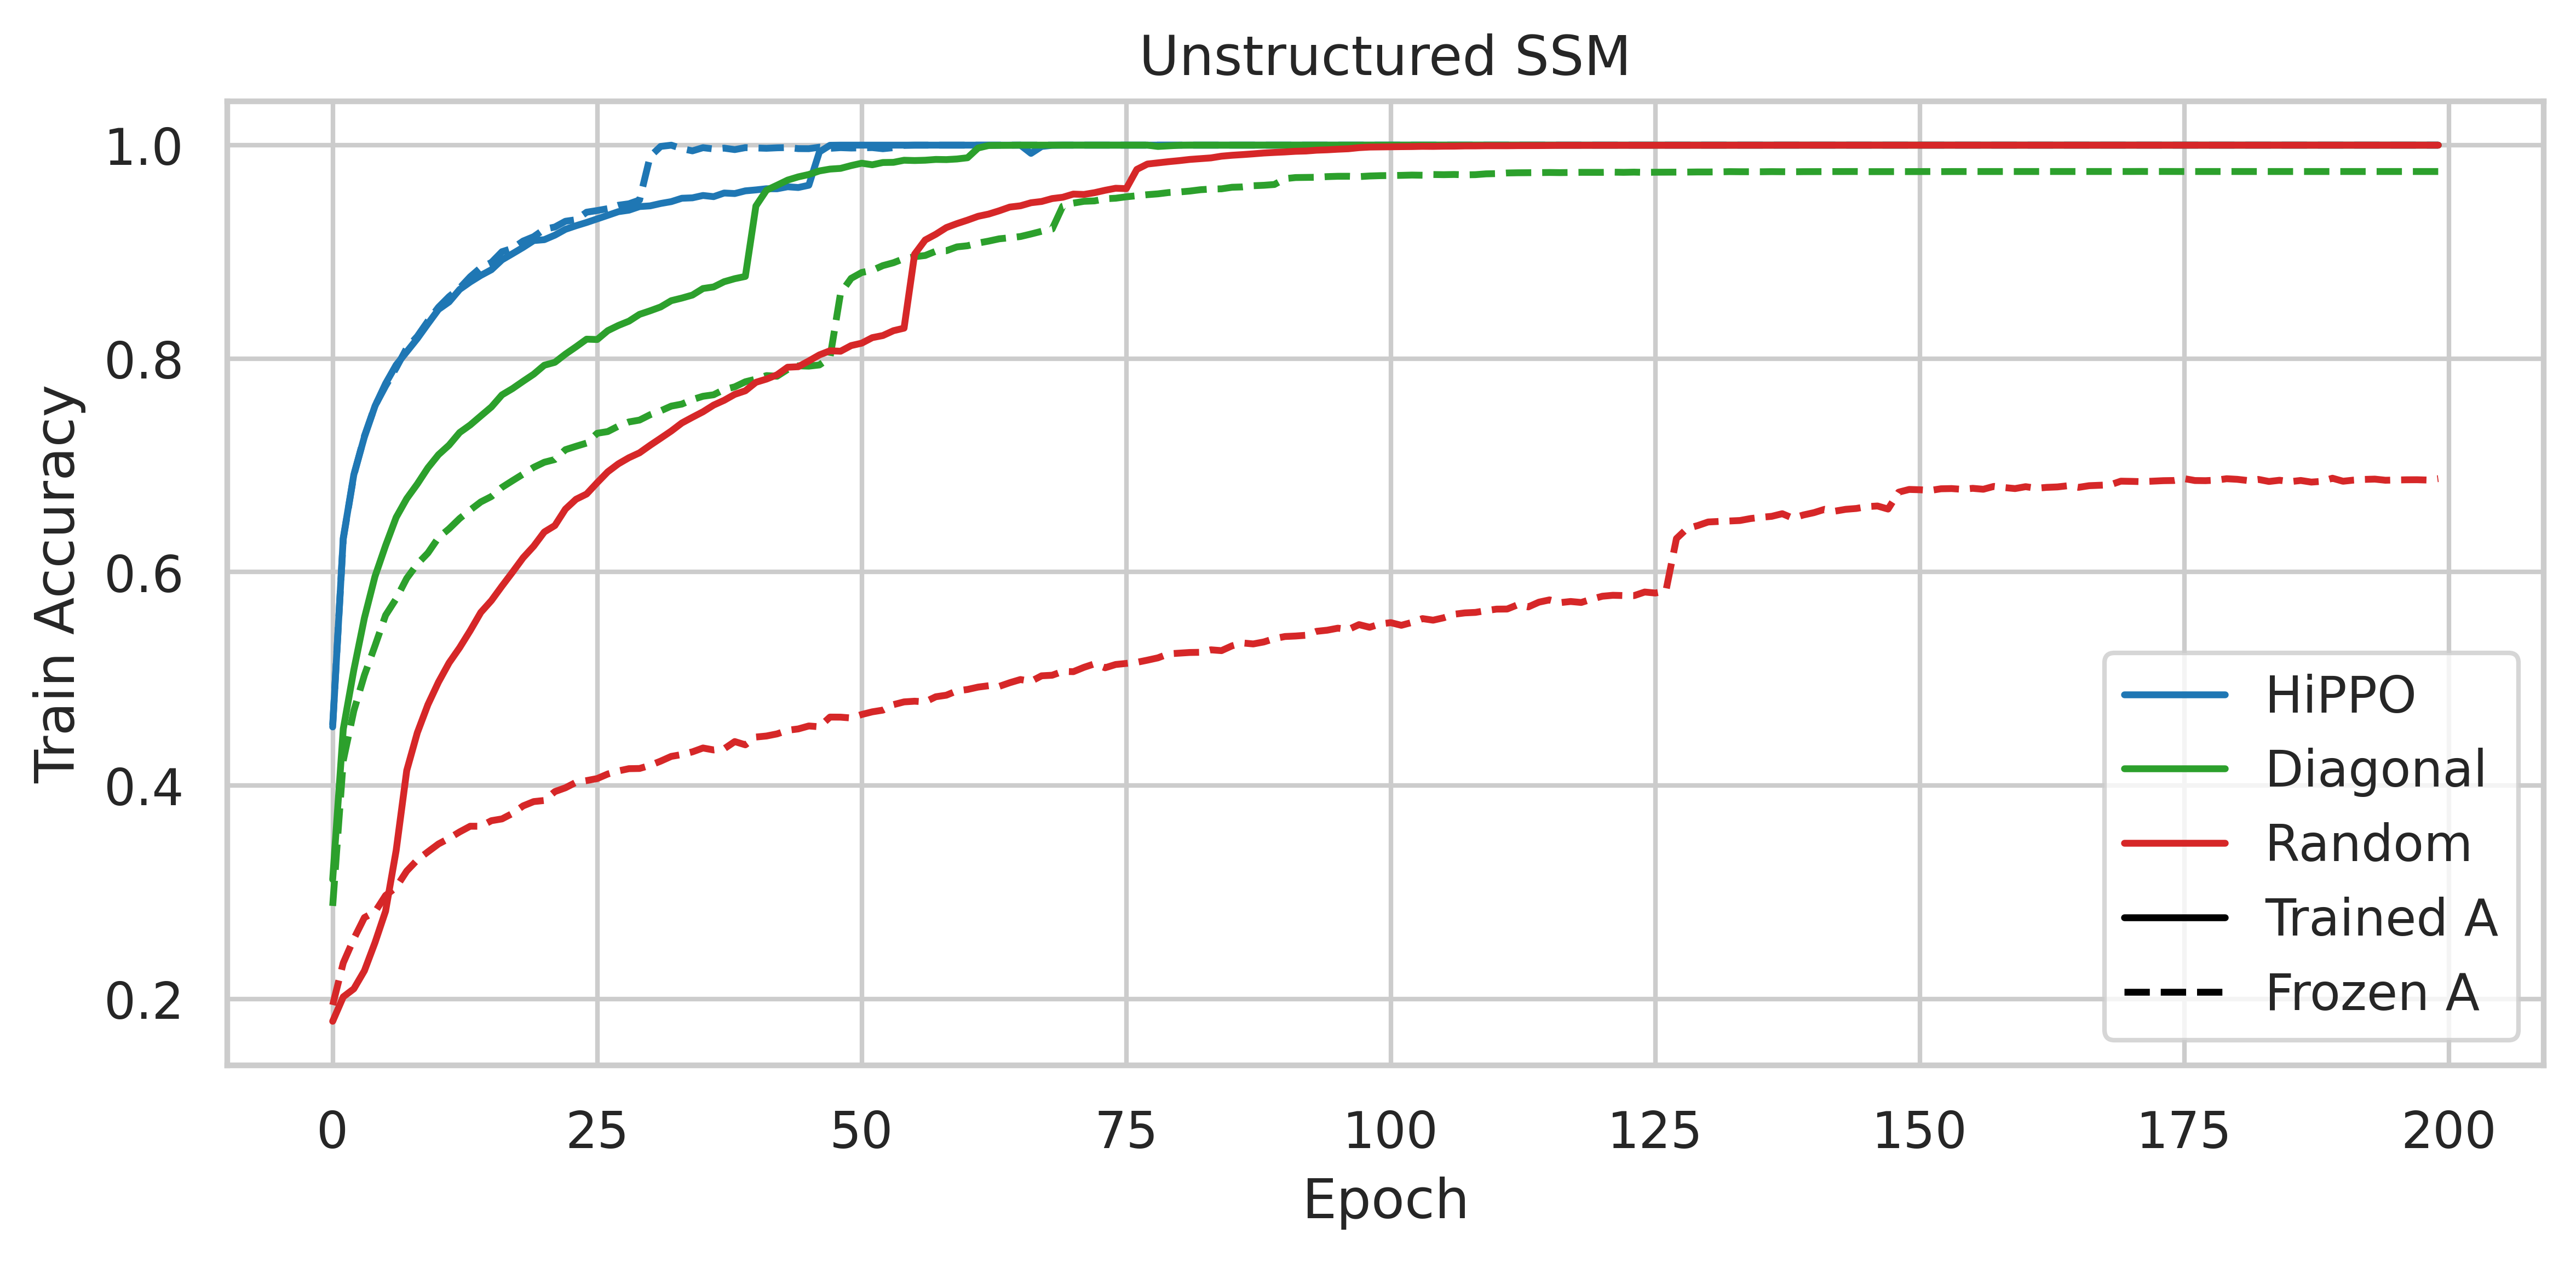
\includegraphics[width=\linewidth]{figs/ssm_ablation_real_train.png}
\end{subfigure}
\begin{subfigure}{.5\linewidth}%
    \centering
    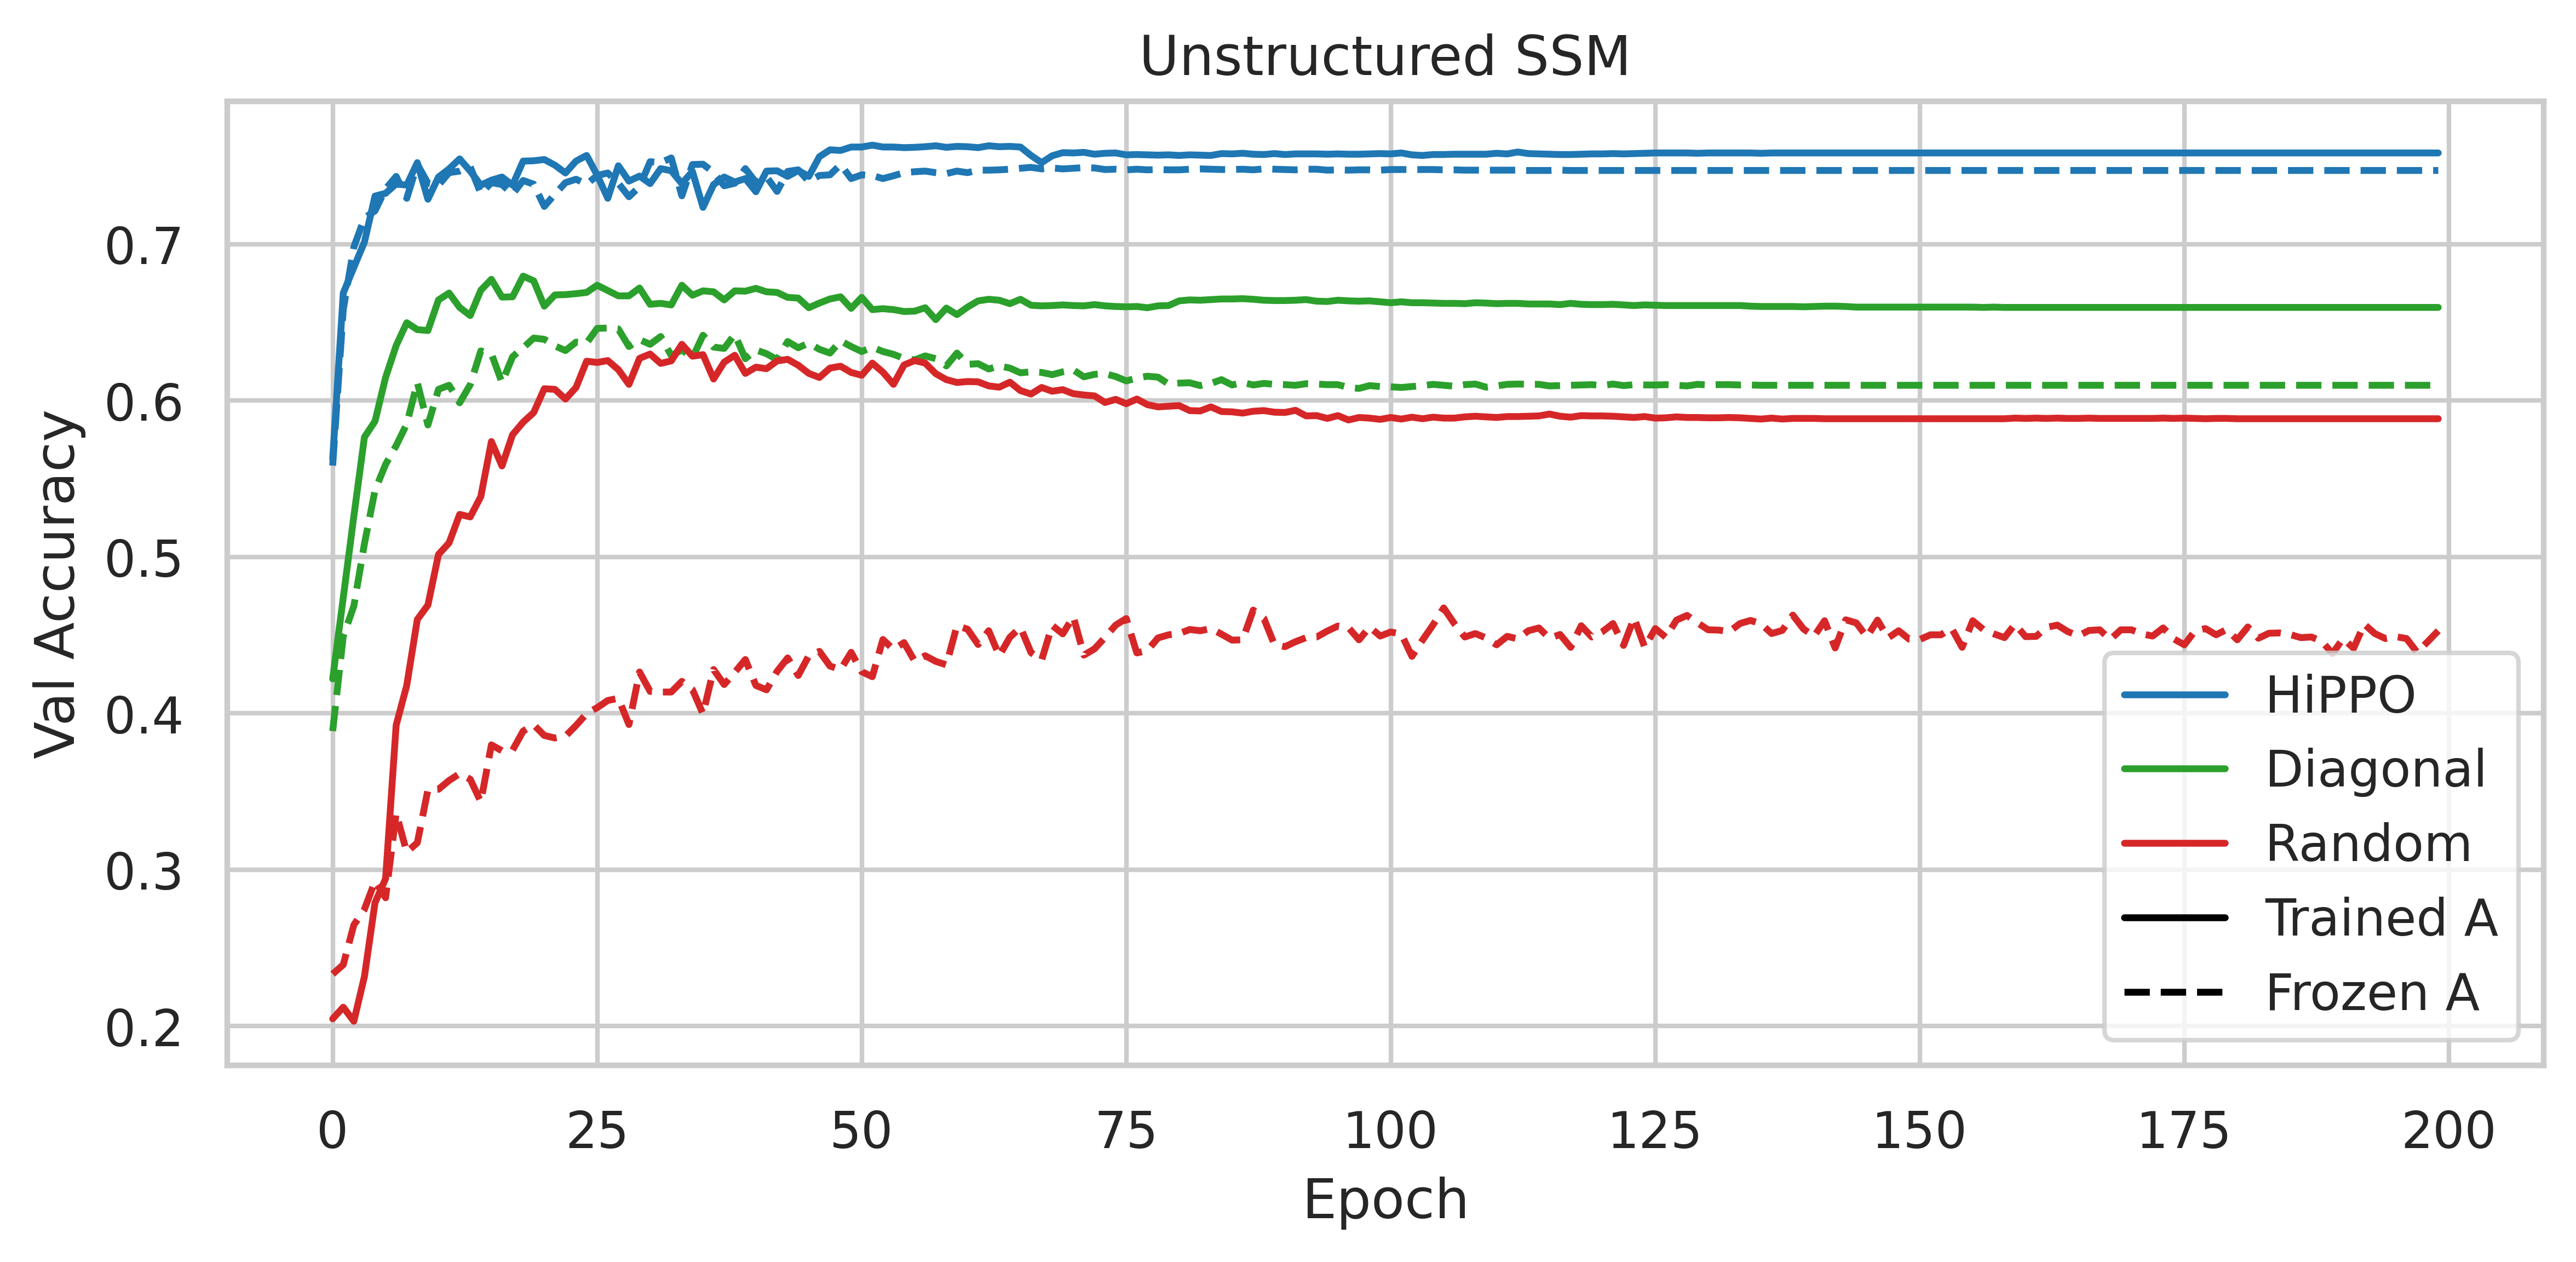
\includegraphics[width=\linewidth]{figs/ssm_ablation_real_validation.png}
\end{subfigure}
\caption{CIFAR-10 classification with unconstrained, real-valued SSMs with various initializations. (\emph{Left}) Train accuracy. (\emph{Right}) Validation accuracy.}
\label{fig:ssm-ablation-real}
\end{figure}

\paragraph{NPLR SSMs.}
The previous experiment validates the importance of HiPPO in SSMs.
This was the main motivation of the NPLR algorithm in S4,
which utilizes structure of the HiPPO matrix \eqref{eq:hippo} to make SSMs computationally feasible.
\cref{fig:ssm-ablation-nplr} shows that random NPLR matrices still do not perform well,
which validates that S4's effectiveness primarily comes from the HiPPO initialization, not the NPLR parameterization.

\begin{figure}[!t]
\begin{subfigure}{.5\linewidth}%
    \centering
    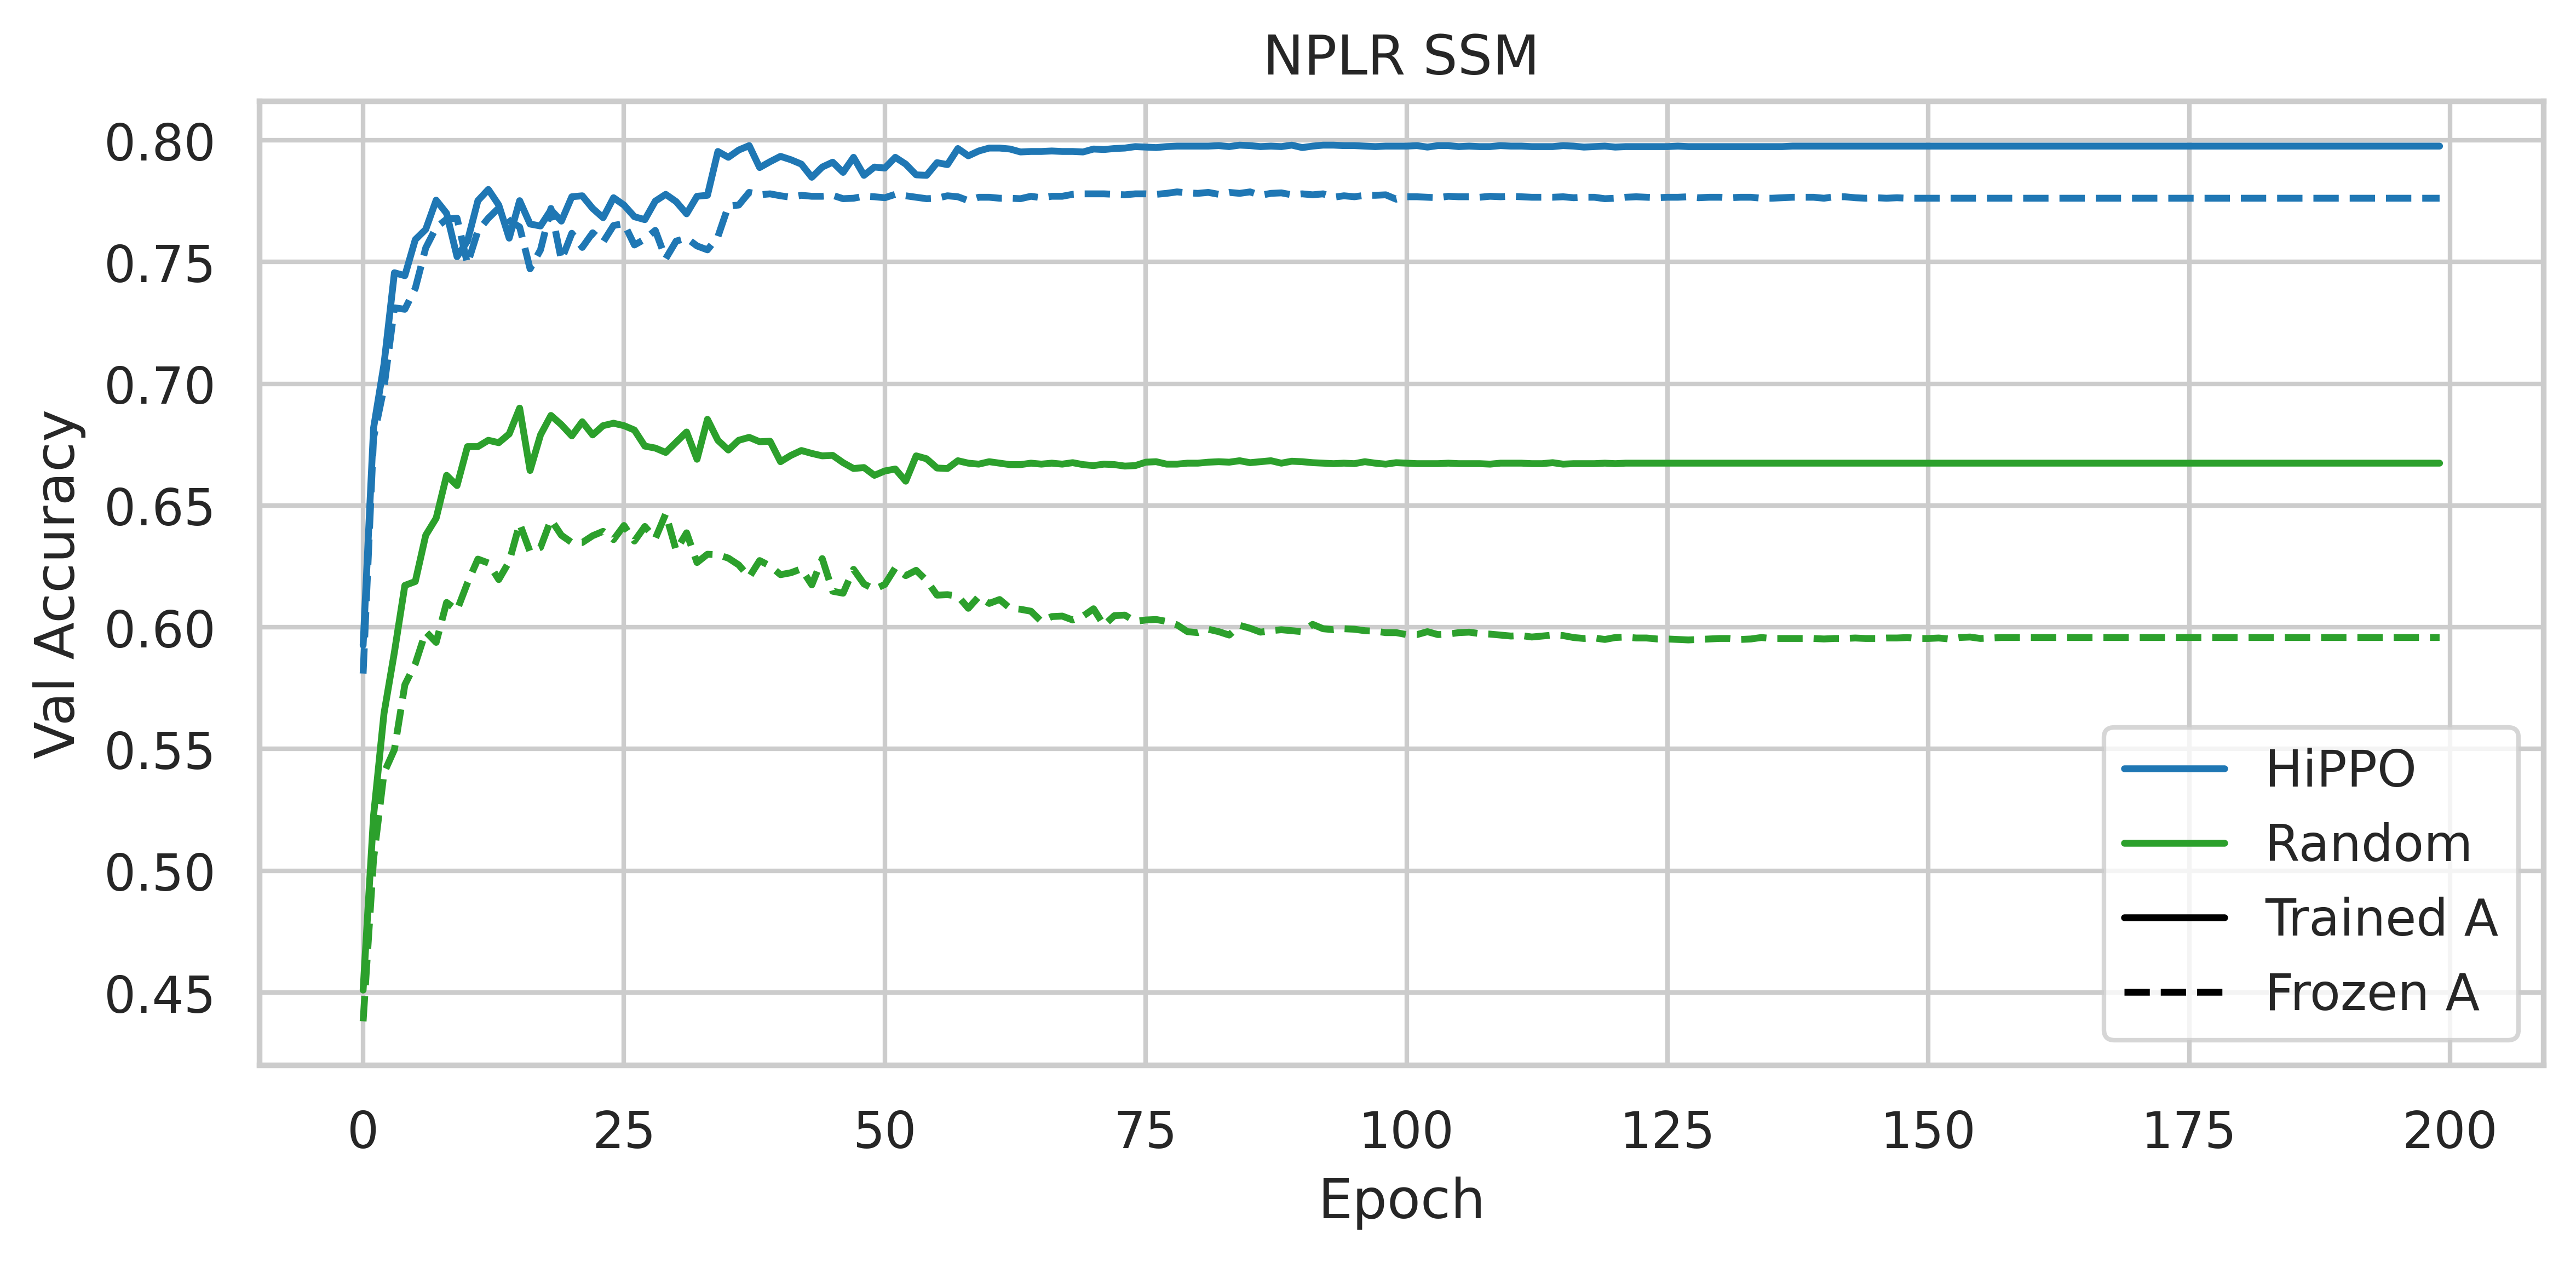
\includegraphics[width=\linewidth]{figs/ssm_ablation_nplr_validation.png}
    \caption{}
    \label{fig:ssm-ablation-nplr}
\end{subfigure}
\begin{subfigure}{.5\linewidth}%
    \centering
    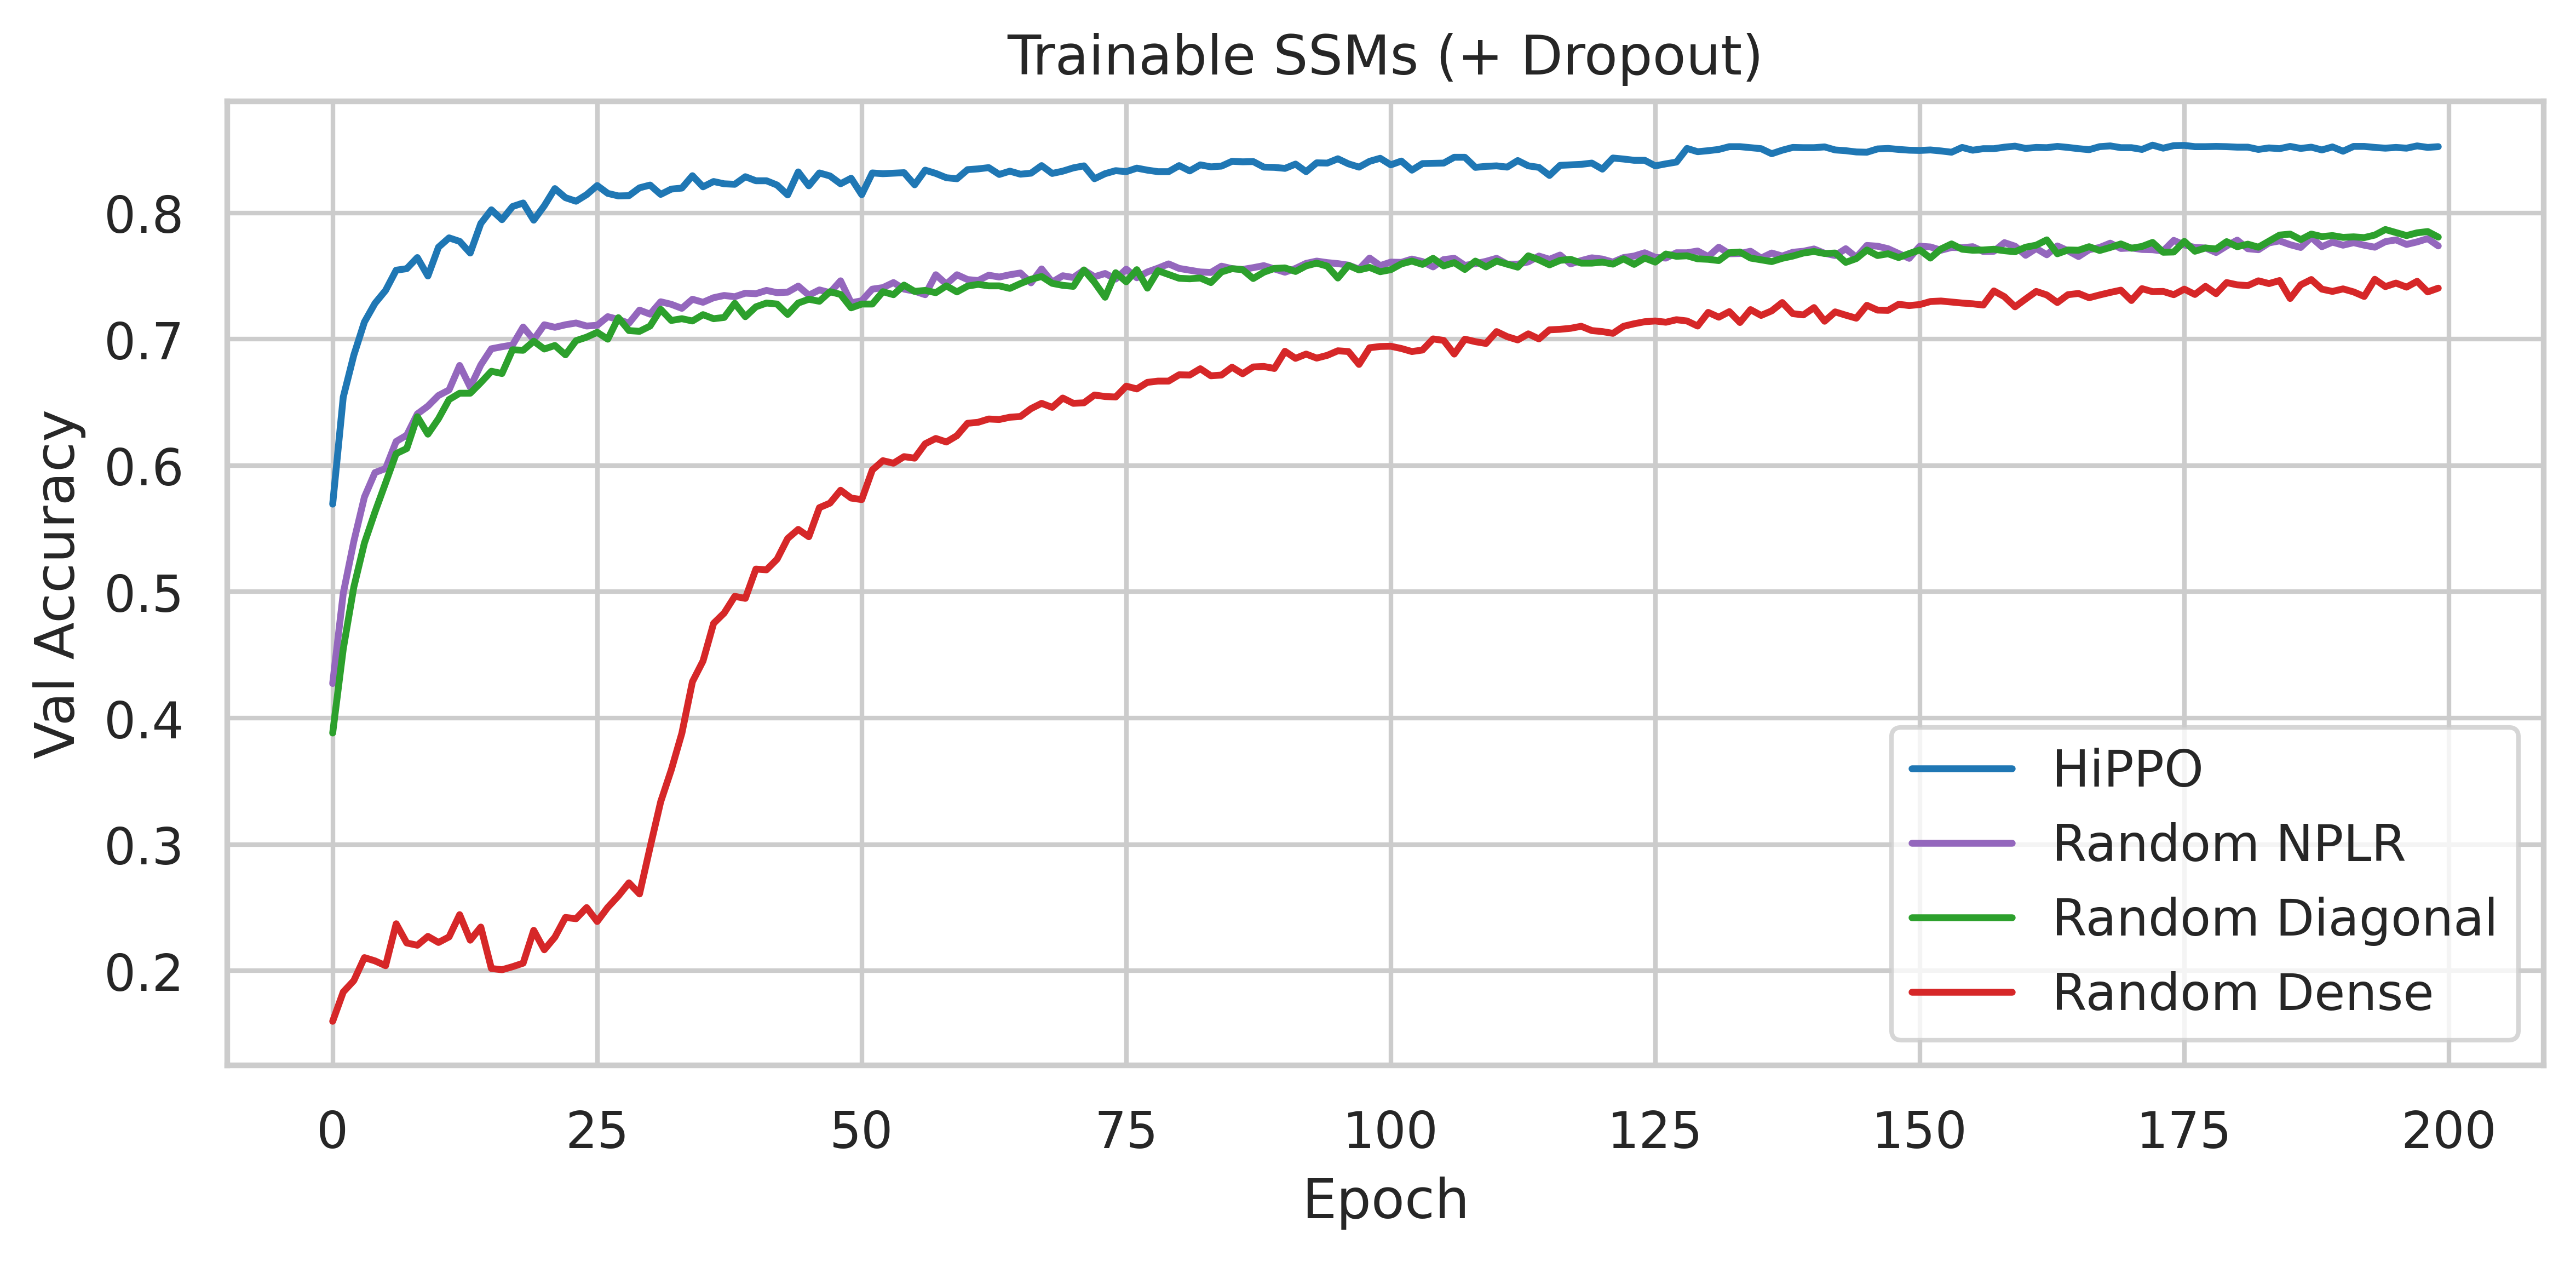
\includegraphics[width=\linewidth]{figs/ssm_ablation_reg.png}
    \caption{}
    \label{fig:ssm-ablation-reg}
\end{subfigure}
\caption{
  CIFAR-10 validation accuracy of SSMs with different initializations and parameterizations.
  (\emph{Left}) NPLR parameterization with random versus HiPPO initialization.
  (\emph{Right}) All methods considered in this section, including minor Dropout regularization. S4 achieves SotA accuracy on sequential CIFAR-10 with just 100K parameters.
}
\end{figure}

Finally, \cref{fig:ssm-ablation-reg} considers the main ablations considered in this section (with trainable SSMs) and adds minor regularization.
With 0.1 Dropout, the same trends still hold, and the HiPPO initialization---in other words, the full S4 method---achieves \( 84.27\% \) test accuracy with just 100K parameters.
